% ==============================================================================
% EE413A
% Lab 2
% The Operational Amplifier
%
% Author:
% Jonas Sjöberg     <tel12jsg@student.hig.se>
% Esther Hedlund    <tfk13ehd@student.hig.se>
% 
% License:
% Creative Commons Attribution-NonCommercial-ShareAlike 4.0 International
% See LICENSE.md for full licensing information.
% ==============================================================================


% ==============================================================================
% INCLUDES AND CONFIGURATION
% ==============================================================================
\documentclass[]{article}

\usepackage[utf8]{inputenc}
\usepackage{siunitx} % Provides the \SI{}{} and \si{} command for typesetting SI
\usepackage{amssymb,amsmath}
\usepackage{graphicx}
\usepackage{longtable,booktabs}
\IfFileExists{microtype.sty}{\usepackage{microtype}}{}

\setlength\parindent{0pt} % Removes all indentation from paragraphs

% ==============================================================================
% DOCUMENT METADATA 
% ==============================================================================
\title{EE413 \\ Lab 005 \\ the Operational Amplifier}
\author{{Jonas Sjöberg} \and {Esther Hedlund}}


\date{}

\begin{document}

\maketitle

\begin{center}
\begin{tabular}{l r}
    Data Performed: & 26 November 2014 \\
    Instructor: TODO
\end{tabular}
\end{center}

% ==============================================================================
% ABSTRACT
% ==============================================================================
\begin{abstract}
"This lab is meant to show the practical use of the operational amplifier in
analog circuit design. Several common circuit configurations will be discussed."
\end{abstract}

\newpage

{
%\hypersetup{linkcolor=black}
\setcounter{tocdepth}{3}
\tableofcontents
}

\newpage

% ==============================================================================
% SECTION: Circuit prototyping setup
% ==============================================================================
\section{Circuit prototyping setup}\label{setup}
The circuit was build on a solderless breadboard, using through-hole parts.
A classic 741 op amp was used with a +/-15V power supply.

% ==============================================================================
% SECTION: Inverting DC Amplifier
% ==============================================================================
\section{Inverting DC Amplifier}\label{inverting-dc-amplifier}
% ==============================================================================

\subsection{Theory}\label{invDC-theory}
% ==============================================================================

\begin{figure}[htbp]
    \centering
        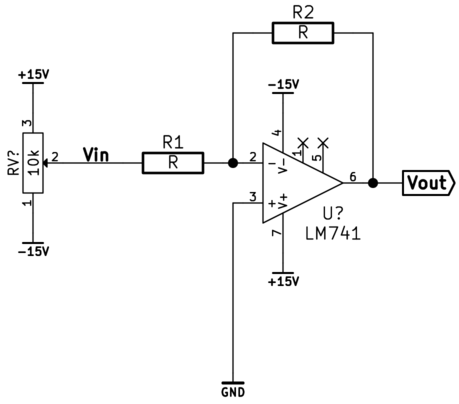
\includegraphics[scale=0.5]{img/invDCamp.png}
    \caption{Inverting DC amplifier}
    \label{fig:invDCamp}
\end{figure}

The basic topology for an inverting amplifier is shown in Figure~\ref{fig:invDCamp}.
Gain $A_v$, can be expressed as a ratio of the feedback impedance to the
input impedance. Op amp action makes the negative input appear as a "virtual earth" summing node. The voltage drops across the resistors scale linearly with their value, and since the op amp compensates to ensure equality in the summing junction, the net effect is an amplified and inverted output.

\begin{equation}
    A_v = \frac{R_2}{R_1}
\end{equation}

The circuit gain for ideal components is therefore;

For $R_2 = 100k\Omega$:

\begin{align} 
A_v     &= \frac{V_{out}}{V_{in}} = -\frac{R_2}{R_1}\\
        &= \frac{100k\Omega}{10k\Omega} = 10\times\\
        &= 20 \times \log{\frac{10}{1}} = 20dB  
\end{align}

For $R_2 = 10k\Omega$:

\begin{align} 
A_v     &= \frac{V_{out}}{V_{in}} = -\frac{R_2}{R_1}\\
        &= \frac{10k\Omega}{10k\Omega} = 10\times\\
        &= 20 \times \log{\frac{1}{1}} = 0dB  
\end{align}

In both cases, the signal phase is inverted $180^\circ$.


\subsection{Measurements}\label{invDC-measurements}
% ==============================================================================

Measured values for the test setup.
\begin{longtable}[c]{@{}lll@{}}
\toprule\addlinespace
$U_{in}$ (V) & $U_{out}$ (V) & $Av$ ($\times$)
\\\addlinespace
\midrule\endhead
-0.103 & +1.087  & -10.35
\\\addlinespace
-1.008  & +10.236   & -10.15
\\\addlinespace
+1.004  & -10.104   & -10.06
\\\addlinespace
\bottomrule
\addlinespace
\caption{$R_2 = 100k\Omega$}
\label{invDCtable1}
\end{longtable}

\begin{longtable}[c]{@{}lll@{}}
\toprule\addlinespace
$U_{in}$ (V) & $U_{out}$ (V) & $Av$ ($\times$)
\\\addlinespace
\midrule\endhead
-0.1003 & +0.112  & -1.116
\\\addlinespace
-1.000  & +1.038   & -1.038
\\\addlinespace
+1.005  & -1.027   & -1.022
\\\addlinespace
\bottomrule
\addlinespace
\caption{$R_2 = 10k\Omega$}
\label{invDCtable2}
\end{longtable}

% Circuit #1
For $R_2 = 100k\Omega$, the actual measured in circuit values of $R_2$ and $R_1$ were 119k$\Omega$ and 11.7k$\Omega$, respectively. Calculated circuit gain for non-ideal, real components;

\begin{align} 
A_v     &= \frac{V_{out}}{V_{in}} = -\frac{R_2}{R_1}\\
        &= \frac{119k\Omega}{11.7k\Omega} = 10.17\times\\
        &= 20 \times \log{\frac{\frac{119k\Omega}{11.7k\Omega}}{1}} = 20.15dB  
\end{align}


% Circuit #2
For $R_2 = 10k\Omega$, the actual measured in circuit values of $R_2$ and $R_1$ were 12.17k$\Omega$ and 11.7k$\Omega$, respectively. Calculated circuit gain for non-ideal, real components;

\begin{align} 
A_v     &= \frac{V_{out}}{V_{in}} = -\frac{R_2}{R_1}\\
        &= \frac{12.17k\Omega}{11.7k\Omega} = 1.04\times\\
        &= 20 \times \log{\frac{\frac{12.17k\Omega}{11.7k\Omega}}{1}} = 0.34dB  
\end{align}

% ==============================================================================
% SECTION: Inverting AC Amplifier
% ==============================================================================
\section{Inverting AC Amplifier}\label{inverting-ac-amplifier}
% ==============================================================================

\subsection{Theory}\label{invAC-theory}
% ==============================================================================

\begin{figure}[htbp]
    \centering
    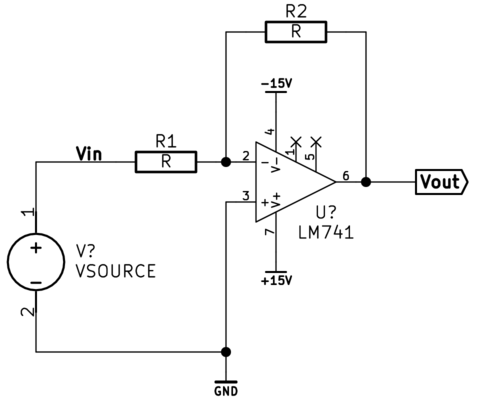
\includegraphics[scale=0.5]{img/invACamp.png}
    \caption{Inverting AC amplifier}
    \label{fig:invACamp}
\end{figure}


The basic topology for an inverting AC amplifier is shown in Figure~\ref{fig:invACamp}.


\begin{equation}
    A_v = 1+\frac{R_2}{R_1}
\end{equation}

The circuit gain for ideal components is;

For $R_2 = 100k\Omega$:

\begin{align} 
A_v     &= \frac{V_{out}}{V_{in}} = -\frac{R_2}{R_1}\\
        &= \frac{100k\Omega}{10k\Omega} = 10\times\\
        &= 20 \times \log{\frac{10}{1}} = 20dB  
\end{align}

For $R_2 = 10k\Omega$:

\begin{align} 
A_v     &= \frac{V_{out}}{V_{in}} = -\frac{R_2}{R_1}\\
        &= \frac{10k\Omega}{10k\Omega} = 10\times\\
        &= 20 \times \log{\frac{1}{1}} = 0dB  
\end{align}

In both cases, the signal phase is inverted $180^\circ$.


\subsection{Measurements}\label{invAC-measurements-1}
% ==============================================================================
Oscilloscope photos in figure~\ref{fig:invACamp20dB_scope} and figure~\ref{fig:invACampunity_scope} show the amplifier input on channel one
the amplifier output on channel two.
Channel two volts/div is set to compensate for the high impedance 10:1 probe setting. 

\subsection{Oscilloscope shots}\label{invAC-oscilloscope-shots}
% ==============================================================================

\begin{figure}[htbp]
    \centering
    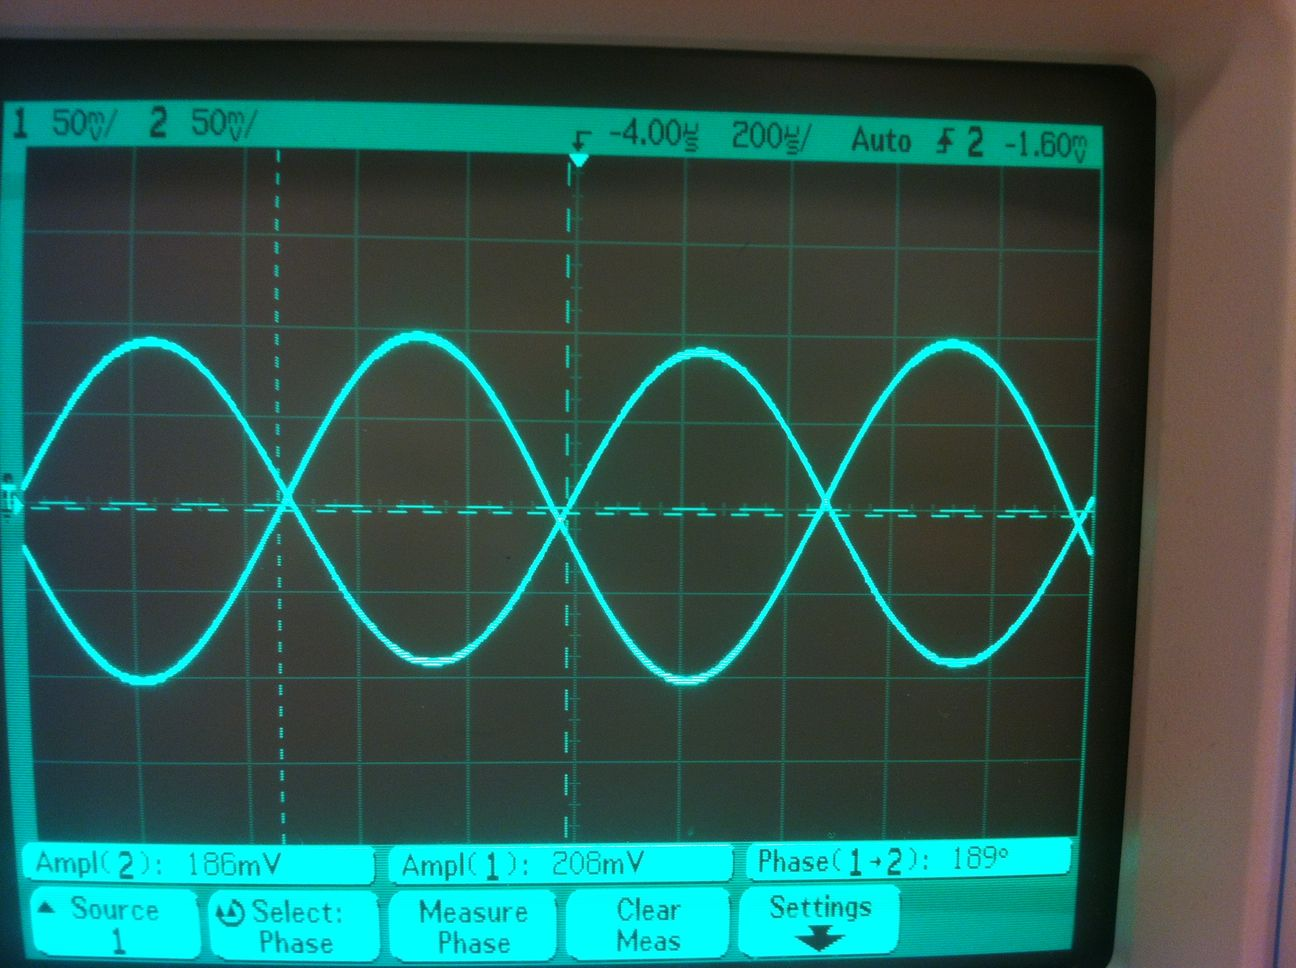
\includegraphics[scale=0.2]{img/invACamp-x10.jpg}
    \caption{Inverting AC amplifier - 20dB gain}
    \label{fig:invACamp20dB_scope}
\end{figure}

\begin{figure}[htbp]
    \centering
    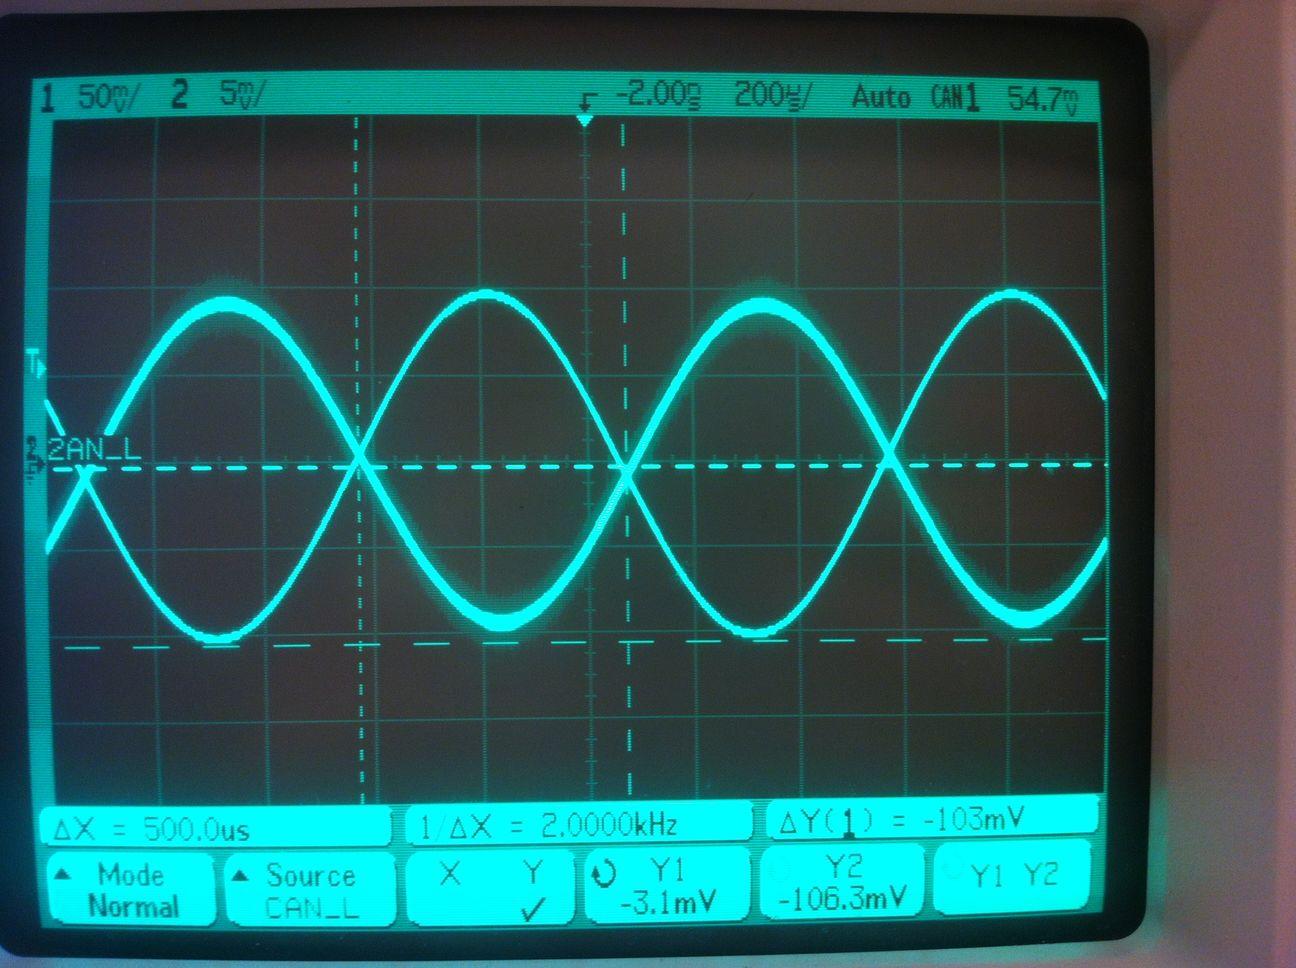
\includegraphics[scale=0.2]{img/invACamp-x1.jpg}
    \caption{Inverting AC amplifier - unity gain}
    \label{fig:invACampunity_scope}
\end{figure}


% ==============================================================================
% SECTION: Non-inverting DC Amplifier
% ==============================================================================
\section{Non-inverting DC Amplifier}\label{non-inverting-dc-amplifier}
% ==============================================================================

\subsection{Theory}\label{noninvDC-theory}
% ==============================================================================

\begin{figure}[htbp]
    \centering
    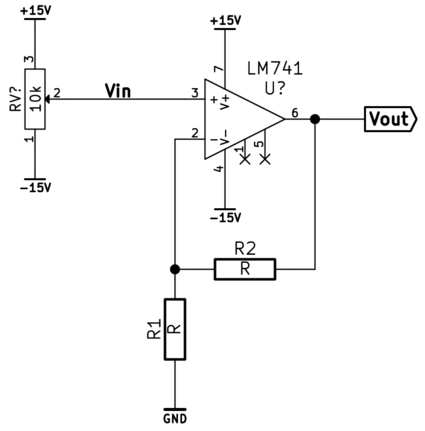
\includegraphics[scale=0.5]{img/noninvDCamp.png}
    \caption{Non-inverting DC amplifier}
    \label{fig:noninvDCamp}
\end{figure}

The basic topology for an non-inverting DC amplifier is shown in Figure~\ref{fig:noninvDCamp}.
Gain $A_v$, is set by the attenuation-factor of the circuit in the feedback-loop. 
A fraction of the output is fed back, causing the op amp to compensate and in effect amplify.

\begin{equation}
    A_v = 1+\frac{R_2}{R_1}
\end{equation}


\subsection{Measurements}\label{measurements-2}
% ==============================================================================

\begin{longtable}[c]{@{}lll@{}}
\toprule\addlinespace
$U_{in}$ (V) & $U_{out}$ (V) & $Av$ ($\times$)
\\\addlinespace
\midrule\endhead
+0.1007 & +0.2164 2 & .15
\\\addlinespace
+1.002 & +2.048 2 & .04
\\\addlinespace
-1.005 & -2.03 2 & .019
\\\addlinespace
\bottomrule
\addlinespace
\caption{$R_2 = 10k\Omega$}
\end{longtable}

\begin{longtable}[c]{@{}lll@{}}
\toprule\addlinespace
$U_{in}$ (V) & $U_{out}$ (V) & $Av$ ($\times$)
\\\addlinespace
\midrule\endhead
+0.1009 & +1.178 & 11.67
\\\addlinespace
+1.1013 & +11.3 & 11.15
\\\addlinespace
-1.004 & -11.09 & 11.05
\\\addlinespace
\bottomrule
\addlinespace
\caption{$R_2 = 100k\Omega$}
\end{longtable}


% ==============================================================================
% SECTION: Non-inverting AC Amplifier
% ==============================================================================
\section{Non-inverting AC Amplifier}\label{non-inverting-ac-amplifier}
% ==============================================================================

\subsection{Measurements}\label{measurements-3}
% ==============================================================================

Input signal amplitude =\\Output signal amplitude =\\Measured
amplification =\\Measured phase =

Theoretical amplification = Theoretical phase =

\begin{figure}[htbp]
\centering
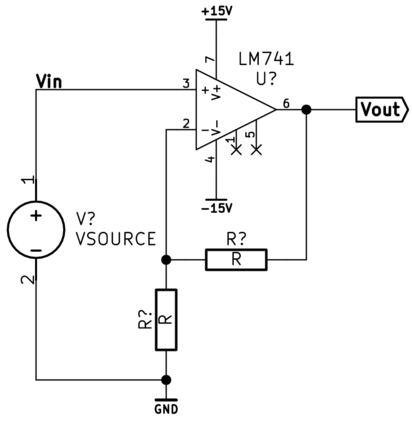
\includegraphics[scale=0.5]{img/noninvACamp.png}
\caption{Non-inverting AC amplifier}
\end{figure}

% ==============================================================================
% SECTION: Active full wave rectifier
% ==============================================================================
\section{Active full wave rectifier}\label{active-full-wave-rectifier}
% ==============================================================================

Active rectifier does not suffer from the ``deadzone'' when the signal
is too small to turn on the rectifying diode. The op amp compensates for
the diode forward voltage drop. The circuit output is a full wave
rectified version of the signal, with a frequency limit mostly set by
the op amp bandwidth. Diode D2 prevents the op amp from hitting the rail
hard when D1 is reverse biased. This makes the recovery and rise time
faster when D1 biases on. This improves circuit response times.

\begin{figure}[htbp]
\centering
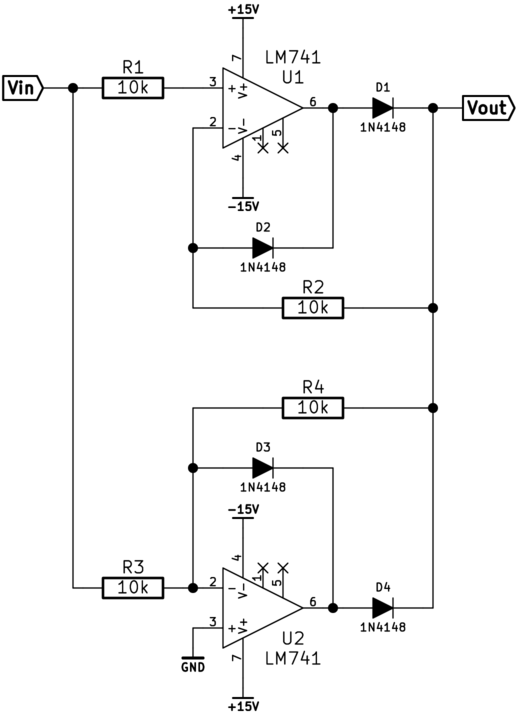
\includegraphics[scale=0.5]{img/fwr.png}
\caption{Active full wave rectifier}
\end{figure}

% ==============================================================================
% SECTION: Results
% ==============================================================================
\section{Results}\label{setup}
% ==============================================================================
TODO

\end{document}
